\chapter{Specification}

	Based on the business requirements we decided that the back-end part of the application must take these five divisions into account: Customers, Employees, Vehicles, Orders and Notifications. In the rest of the chapter we are describing features that these modules should have.
	
	\section{Customers}
		Customers are uniquely identified by telephone number. We also want to store about each of them these information:
		\begin{itemize}
			\item ID
			\item Name
			\item Note
			\item Fraud status
		\end{itemize}
		With Customer entity we are able to do these operations:
		\begin{itemize}
			\item Create and confirm
			\item Update
			\item Destroy
			\item Recover password
			\item Login and logout
			\item List favourite locations
			\item List all customers and show specific customer
		\end{itemize}
		\subsection{Operation create and confirm}
			There are two ways how customer can be created. It is either directly through registration or indirectly by creating new order.
			
			Directly registered customers are created in exchange for telephone number, password and optional name. With this type of account customer can later login with provided password. Application must verify given telephone.
			
			Indirectly registered user is created during creation of new order for telephone number, which doesn't belong to any existing customer. This customer type is just envelop for the purpose of tracking information and statistics - mostly for better customer support. This account type can not be used for authentication. Indirectly registered user can be directly registered later without any difference to normal direct registration.
		
		
		\subsection{Operation update}
			Customer can update only it's own name and password. Employees are able to change any customer's name, note and fraud status.
		\subsection{Operation destroy}
			Destroy the customer can be invoked by that customer or the administrator. Orders made by that customer are not deleted - the order has no customer then.
		\subsection{Operation password recovery}
			In case of lost password is customer able to recover it. At first customer asks for the recovery with its telephone. In return it receives recovery token via SMS. This token is valid for 5 minutes. With this token and telephone number can new password be set. Customer is able to ask for token resend - which will invalidate last token, generate new token and sends it via SMS.
		\subsection{Operation login and logout}
			With login operation we receive login token in exchange for telephone number and password. We send this token with each request to be authenticated.
			Customer can login if and only if it is directly registered and confirmed.
			Logout just invalidates the session - customer must log in again to be authenticated.
		\subsection{Operation list favourite locations}
			Our application must provide list of customer favourite places. In the front-end part of the application should be this implemented in the part where customer chooses its pick-up and drop-off location. 
			
			Main priority is to provide list of these places fast = less than one second. Most important are first five returned places and the most likely places based on current conditions should be among them These places should be ordered with respect to the given location ( in reality current customer location or pick-up location when choosing drop-off ). It should also take into account whether customer chooses pick-up or drop-off. These recommendations should be based on customer's order history and respect start - finish relation of the orders. 
			
			Let's imagine customer that has two routes - it often goes from pub to its home and sometimes goes from its home to gym. Application then should return its home as first item when looking for drop-off recommendation from unknown pick-up place. Application should also return gym as first item when user is asking for drop-off recommendation with pick-up at home, even though pub is much more frequent place in its history.
			
			 Show the favourite locations list of a specific user is permitted only for that specific user or any employee.
		 
		\subsection{Operation list all customers and show specific customer}
			Our API must provide information of the customers created in our application.
			Show specific customer's data is available only for the customer itself or any employee. 
			
			List all the customers is available for administrator only, because the list of the customers is one of the most valuable asset of the taxi company and we don't want to provide it for the staff. Of course the employee could get all the customers by going one by one via operation show, but it takes more time so this is for our purpose enough.
		
	\section{Employees}
		There three types of employees - administrators, dispatchers and drivers. Employees unlike customers are identified via email. We store these information about each one:
		\begin{itemize}
			\item Email
			\item Name
			\item Photograph
		\end{itemize}
		
		In our application we also have information about the employees shifts - whether it is at work or not. For drivers we also process current locations and their order queues. 
		
		Operations on employees are almost the same as operations on customers. Operations differs mainly in permissions. 
		\begin{itemize}
			\item Create and confirm
			\item Update
			\item Destroy
			\item Recover password
			\item Login and logout
			\item List all employees and show specific employee
		\end{itemize}
		
		\subsection{Shifts}
		 Employees could be in three statuses: 
			\begin{itemize}
				\item available
				\item unavailable
				\item pause
			\end{itemize}
			Available means that the employee is on site and can handle orders. Unavailable is when it is not at work. Pause status is there for the situations when the employee knows that it won't be available for a while but wants to finish its orders.
			
			Switching directly from available to unavailable should be only in cases of emergency, e.g. driver has flat tire and cannot continue. Employees will be instructed not to do so for better customer experience. 
			
			Employee is available to list the history of its shifts and administrator is available to list shifts for all the employees. Changing shifts (available statuses) are employees allowed only for themselves.
		
		\subsection{Driver locations}
			Each driver from the shift start until the shift end sends at regular intervals its location. Driver's current location is able to set only driver itself. Get the last  driver's location is can anyone, so the front-end can display the current location of arriving driver even for anonymous customer. 
		
		\subsection{Driver order queues}
			Each driver has a queue of orders that are assigned to it. Administrator can see all the queues, driver can see only its own queue.
	
		\subsection{Operation create and confirm}
			Employee can be created by administrator only. In exchange for the email, optional name and image the confirmation email is sent to the employee. Then the employee is by clicking the link in email redirected to front-end page, where it fill its password. The link contains confirmation token which will the front-end together along with the optional name and image send to our application.
	
		\subsection{Operation update}		
		Employee can update its password, name and image. Administrator can besides these fields change also employee role.
		\subsection{Operation destroy}
		Only administrator can remove the employee from the application. When the employee is removed, all the shifts and driver queue is removed too. Orders associated with the employee remains in system but the corresponding employee field is removed.
		\subsection{Operation recover password}
		Recovering the forgotten password is exactly the same as in the customers case - except the reset password token is sent via email in link to the front-end.
		\subsection{Operation login and logout}
		Only difference in these operations between the employees and customers is that the employees login with email instead of telephone number. Everything else is the same.
		\subsection{Operation list all employees and show specific employee}
		Show all the employees or specific employee can only administrators and dispatchers. The rest (drivers, customers, anonymous users) can see only drivers who are on shift.
		
		There is also different attributes which are shown for different people. Public attributes that anyone can see are id, name and image of the employee. Email, roles, and other attributes like timestamps of creation or update are available only to employee itself, dispatchers or administrators.
	
	\section{Vehicles}
		Taxi company has the vehicle fleet we want to have in our system too. Each driver's shift starts with selecting the vehicle driver will ride in, so the customer can see and choose the car that fit its needs.
		
		 For each vehicle we have these information:
		\begin{itemize}
			\item name
			\item internal vehicle number for taxi company used for communication
			\item plate
			\item image
			\item how many customers can fit in - required
			\item whether the vehicle is available for driving or not e.g. is temporarily in the car repair shop
		\end{itemize}
		These operations with vehicles our application supports:
		\begin{itemize}
			\item Create and update
			\item Show all and specific
			\item Destroy
		\end{itemize}
		\subsection{Operation create, update and destroy}
			Only administrators can create, update and destroy company's vehicles. They can manipulate all the specified information. When the car is deleted, all the corresponding shifts or orders will have set the null value instead of the vehicle.
		\subsection{Operation show all and specific vehicle}
			Administrators can see all the vehicles, others can see only the active ones. 
			
			Operations show to anyone all the attributes besides the internal vehicle number and the availability. Employees can see all of the attributes.
	\section{Orders}
	 	Order is key entity in this application. Each order must go through process from creation to successful finish or cancellation. About each order we would like to have these information:
		
		\begin{itemize}
			\item id
			\item status 
			\item driver who takes care of it
			\item vehicle by which it is processed with
			\item pick-up and drop-off location coordinates and addresses
			\item passenger count
			\item note
			\item contact telephone in case the customer is ordering for someone else
			\item estimated price
			\item whether the assigned driver can not be changed (is explicitly chosen)
			\item VIP (just internal flag for the taxi company)
			\item flight number - in case that the order is to/from the airport
			\item customer
			\item assigned dispatcher
			\item date and time when the customer wants the taxi to arrive to the pick-up location
			\item source - whether it was created by dispatcher or directly by customer via front-end application
		\end{itemize}
		Also with order we want to know these information about times. In parenthesis are the terms how the times will be referenced in the whole thesis and application:
		\begin{itemize}
			\item created time
			\item application estimate when the driver starts arriving to customer (start est.)
			\item when the driver started arriving to customer (start)
			\item estimation when will the driver arrive to the customer (arrived time est.)
			\item actual time when driver arrived to the customer - (arrived time)
			\item estimation and actual time when the driver has picked up  customer and starts driving to the drop-off destination (picked-up time est., picked-up time)
			\item finish time estimation and actual finished time(finish time, finish time est.)
		\end{itemize}
		
		These actions can be performed:
		\begin{itemize}
			\item create
			\item show all / specific
			\item my orders for dispatcher
			\item driver arrivals
			\item confirm by driver
			\item refuse
			\item arriving
			\item change arrive time
			\item arrived
			\item customer not on its place
			\item picked up
			\item change drop off time
			\item change drop off location
			\item finished
			\item fraud
			\item unfraud and process
			\item cancel
		\end{itemize}
		
		
		
		Because the order process Illustration displaying all the order statuses, actions what we can do with the order and actions which must our system do.
		\begin{figure}[h]\centering
			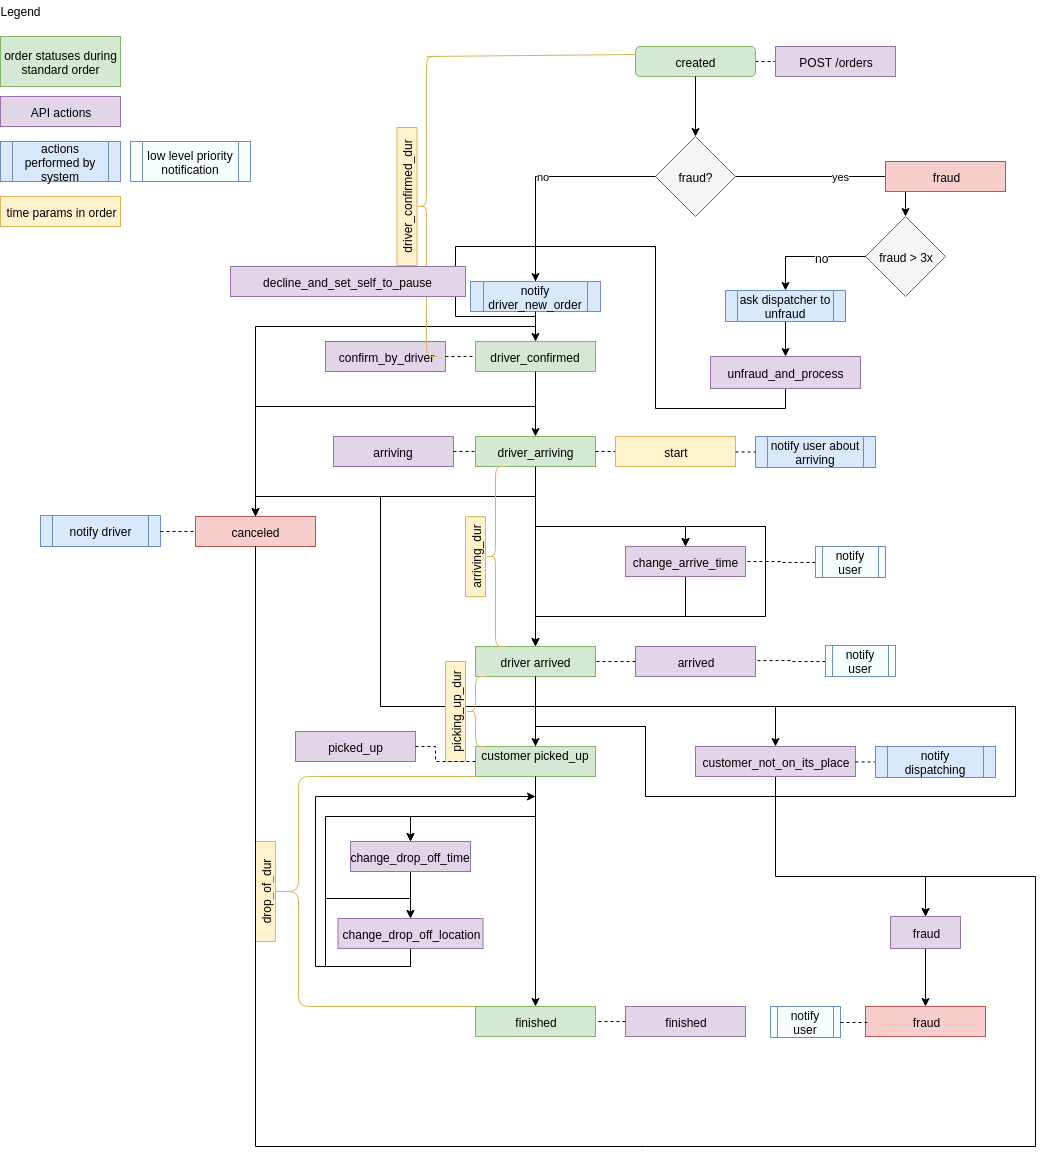
\includegraphics[width=\textwidth]{orders/order_process_scheme.png}
			\caption{Order process scheme}\label{order-process-scheme}
		\end{figure}
	
		\subsection{create}
		
		\subsection{show all\/specific}
		\subsection{my orders for dispatcher}
		\subsection{driver arrivals}
		\subsection{confirm by driver}
		\subsection{arriving}
		\subsection{change arrive time}
		\subsection{arrived}
		\subsection{customer not on its place}
		\subsection{picked up}
		\subsection{change drop off time}
		\subsection{change drop off location}
		\subsection{finished}
		\subsection{fraud}
		\subsection{unfraud and process}
		\subsection{cancel}
	
	\section{Notifications}
